%%% Preamble
\documentclass[paper=a4, fontsize=11pt]{scrartcl}
\usepackage[T1]{fontenc}
\usepackage{fourier}

\usepackage[brazil]{babel}
\usepackage[protrusion=true,expansion=true]{microtype}	
\usepackage{amsmath,amsfonts,amsthm} % Math packages
\usepackage[pdftex]{graphicx}	
\usepackage{subcaption}
\usepackage{url}
\usepackage[small,compact]{titlesec}

\usepackage[margin=3cm]{geometry}
% showframe% <- only to show the page layout
\usepackage{natbib}
\usepackage{dirtree}
\usepackage{listings}
\usepackage{color}
%%% Custom sectioning
\usepackage{sectsty}
\allsectionsfont{\centering \normalfont\scshape}

%%% Custom headers/footers (fancyhdr package)
\usepackage{fancyhdr}
\pagestyle{fancyplain}

\fancyfoot[L]{IPEA - DISET}											% Empty
\fancyfoot[C]{\projectname}											% Empty
\fancyfoot[R]{\thepage}									% Pagenumbering
\renewcommand{\headrulewidth}{0pt}			% Remove header underlines
\renewcommand{\footrulewidth}{0pt}				% Remove footer underlines
\setlength{\headheight}{13.6pt}


%%% Equation and float numbering
\numberwithin{equation}{section}		% Equationnumbering: section.eq#
\numberwithin{figure}{section}			% Figurenumbering: section.fig#
\numberwithin{table}{section}				% Tablenumbering: section.tab#


%%% Maketitle metadata
\newcommand{\horrule}[1]{\rule{\linewidth}{#1}} 	% Horizontal rule
\newcommand{\projectname}{Indicador de Tecnologias Emergentes}
\title{
		%\vspace{-1in} 	
		\usefont{OT1}{bch}{b}{n}
		\normalfont \normalsize \textsc{IPEA - DISET} \\ [25pt]
		\horrule{0.5pt} \\[0.4cm]
		\huge \projectname \\
		\horrule{2pt} \\[0.5cm]
}
\author{
		\normalfont 								\normalsize
        Fred Guth\footnote{consultor contratado.}\\[-3pt]		\normalsize
        \today
}
\date{}


%%% Begin document
\begin{document}
\maketitle
\thispagestyle{empty}
\section{Objetivo}
Antecipar tecnologias emergentes com maior potencial de impacto é essencial para um bom planejamento de políticas públicas.  Usualmente, essa atividade é bastante qualitativa, se baseando no conhecimento de especialistas e na análise de patentes e artigos científicos. Entretanto, redes sociais passaram a expressar, em tempo real, a opinião de diferentes agentes econômicos, incluindo empresas, institutos de pesquisa e publicações especializadas em tecnologias emergentes; tornando possível mensurar quantitativamente, pelo número de menções, o julgamento agregado dessa multidão de agentes  do potencial de tecnologias (assumindo-se que os agentes mencionam mais as tecnologias em que mais vêem potencial). É um fenômeno bem relatado \citep{surowiecki2004wisdom} que julgamentos agregados deste tipo produzem boas previsões.

Neste projeto, usamos processamento de linguagem natural para criar um indicador quantitativo para tecnologias emergentes mencionadas no Twitter por contas previamente selecionadas.

\section{Metodologia}
O processo de construção do \textbf{Indicador de Tecnologias Emergentes (ITE)} abrange as seguintes etapas:
\begin{enumerate}
	\item Captura dos tweets\footnote{A curadoria das contas e a captura dos \emph{tweets} foram realizadas previamente e fogem do escopo do presente projeto.}
	\item Análise exploratória dos dados
	\item Limpeza dos dados e definição dos tópicos
	\item Construção da matriz de frequências Semestre-Tópico
	\item Detecção estatística de anomalias
	\item Geração do Indicador
\end{enumerate}
\subsection{Análise exploratória dos dados}
A análise exploratória de dados (AED) é uma abordagem de análise com objetivo de capturar um panorama geral dos dados com métodos visuais. No presente projeto, a AED não foi estensiva, até mesmo porque a maior variabilidade dos dados está no texto dos tweets o que não é capturado pela mesma. Entretanto, a AED foi importante para identificar potenciais problemas com diferentes abordagens estatísticas. Os resultados da AED serão apresentados na seção \ref{sec:dados}.
\subsection{Limpeza dos dados e definição dos tópicos}
\subsubsection{Limpeza}
A limpeza dos dados tem como objetivo padronização e a remoção de termos anômalos indesejados na análise. Todas as ações de limpeza são opcionais e podem ser \emph{desligadas} a partir de um arquivo de configuração (ver \ref{config.ini}).
\begin{itemize}
	\item  remoção de acentos
	\item  remoção de \emph{hashtags} e menções a contas do twitter: apesar de hashtags serem um sinal forte de importância no Twitter, achamos importante dar a opção de fazer a análise sem hashtags.
	\item  remoção de URLs
	\item  remoção de números: palavras contendo apenas números, por exemplo "2017" é removido, enquanto "23andme" não é.
\end{itemize}
\subsubsection{Definição dos tópicos}
Qualquer palavra usada em um \emph{tweet} do corpus é, inicialmente, considerada um tópico, uma vez que, a priori, não temos como saber que uma palavra está no contexto de tecnologia. Pior do que isso, além dos termos individuais, \textbf{uni-gramas}, como analisamos também \textbf{bi-gramas}, combinações de duas palavras. No limite o número de tópicos pode ser quadrático em relação ao tamanho do vocabulário do corpus.

Tendo em vista que nosso corpus contém apenas mensagens curtas, o contexto em que termos tecnológicos aparecem não são muito identificáveis. Em outras palavras, queremos encontrar um pequeno sinal em um grande mar de ruído. Essa característica do problema nos leva a focar primeiro em identificar anomalias em geral, que podem ou não ser tecnológicas, deixando o problema da categorização dos tópicos como secundário.

Um primeiro passo é, então, reduzir o tamanho do vocabulário considerado. Parte disso é feito pela própria limpeza, mas consideramos também que palavras devem ter um número mínimo de menções-dia\footnote{menção-dia é frequencia de menções em diferentes dias, ou seja, várias menções no mesmo dia contam como uma.}. Além desses filtros, também estabelecemos um limite (\emph{dict\_size}) no tamanho do dicionário, pegando apenas as \emph{dict\_size} palavras com mais menções-dia no corpus.

Também filtramos \emph{stop words}, que são palavras comuns. Todas as principais bibliotecas de NLP possuem uma lista de \emph{stop words} do idioma inglês. Utilizamos a lista da biblioteca NLTK \citep{nltk} e adicionamos uma lista própria de \emph{stop words} que pode ser alterada no arquivo de configuração (\S \ref{config.ini}). Tal lista foi criada especificamente para o desafio deste projeto e parte da constatação que mesmo contas especializadas engajam-se em assuntos da cultura e capturam o zeitgeist ao longo do tempo.

\subsection{Matriz de frequências Semestre-Tópico}
\begin{figure}[h]
	\centering
	\caption{Matriz de frequências Semestre-Tópico.}
	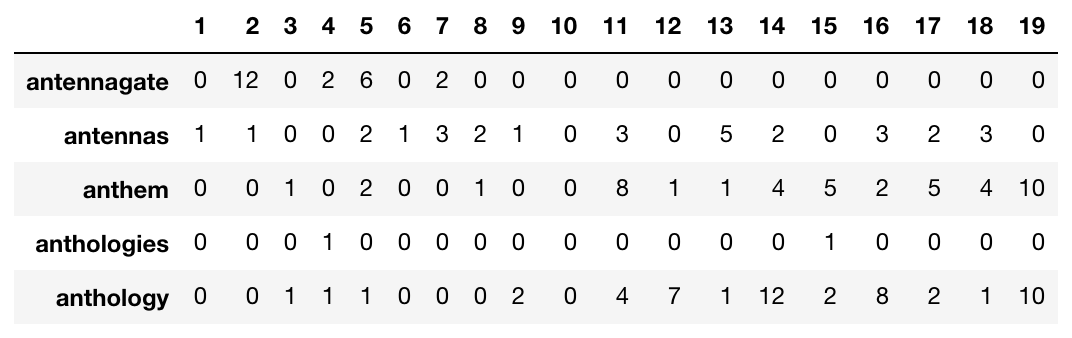
\includegraphics[width=.8\columnwidth]{sem-term}
	\label{fig:sem-term}
\end{figure}

A matriz semestre-tópico é uma matriz que descreve a frequencia de palavras que ocorrem semestre a semestre. É como uma matriz \emph{document-term} onde o documento é o conjunto agregado de \emph{tweets} de um semestre. 
Um dos problemas do nosso corpus que é possível verificar na Figura \ref{fig:volume-tweets}, é que o número de mensagens coletadas por semestre é bastante diverso e essa variação poderia afetar nosso modelo estatístico. Nesse contexto, é preciso normalizar a frequência pelo número de mensagens por semestre.
\subsection{Detecção estatística de anomalias}
Neste trabalho, ossa principal ferramenta para detecção de anomalias é a distribuição de Poisson, que expressa a probabilidade de uma série de eventos ocorrer em um período, dado que um evento em qualquer intervalo independe da probabilidade dele acontecer em qualquer outro intervalo.

No nosso caso, os eventos não são exatamente independentes, porque quando uma determinada conta no \emph{Twitter} com autoridade começa a abordar um tópico, desperta o interesse de outras contas. Mas esse é justamente o caso que queremos identificar, ou seja, nossas anomalias são casos em que a distribuição de Poisson não explica a distribuição de tópicos no \emph{Twitter} que observamos.

Seja o momento inicial das observações $t=0$ e $N(t)$ o número de eventos que ocorrem até uma certa data $t$, um processo estocástico de Poisson pode ser descrito como:
\begin{align}
	P[N(t)=K]=\frac{e^{-\lambda t} (\lambda t )^k}{k!},\,\! \label{poisson}
\end{align}
onde $\lambda$ representa o número de eventos por período esperado (a "velocidade"  do período anterior no nosso caso).
Em nossos experimentos, os primeiros 1000 uni-gramas apresentaram probabilidade de ocorrência segundo (\ref{poisson}) inferior a 0.15\% e no caso de bigramas, inferior a 0.03\%.

\subsection{Geração do Indicador}

\section{Dados}\label{sec:dados}
\begin{figure}[!h]
  \centering
  \begin{minipage}[t]{0.4\textwidth}
		\caption{Tweets por fonte.}
		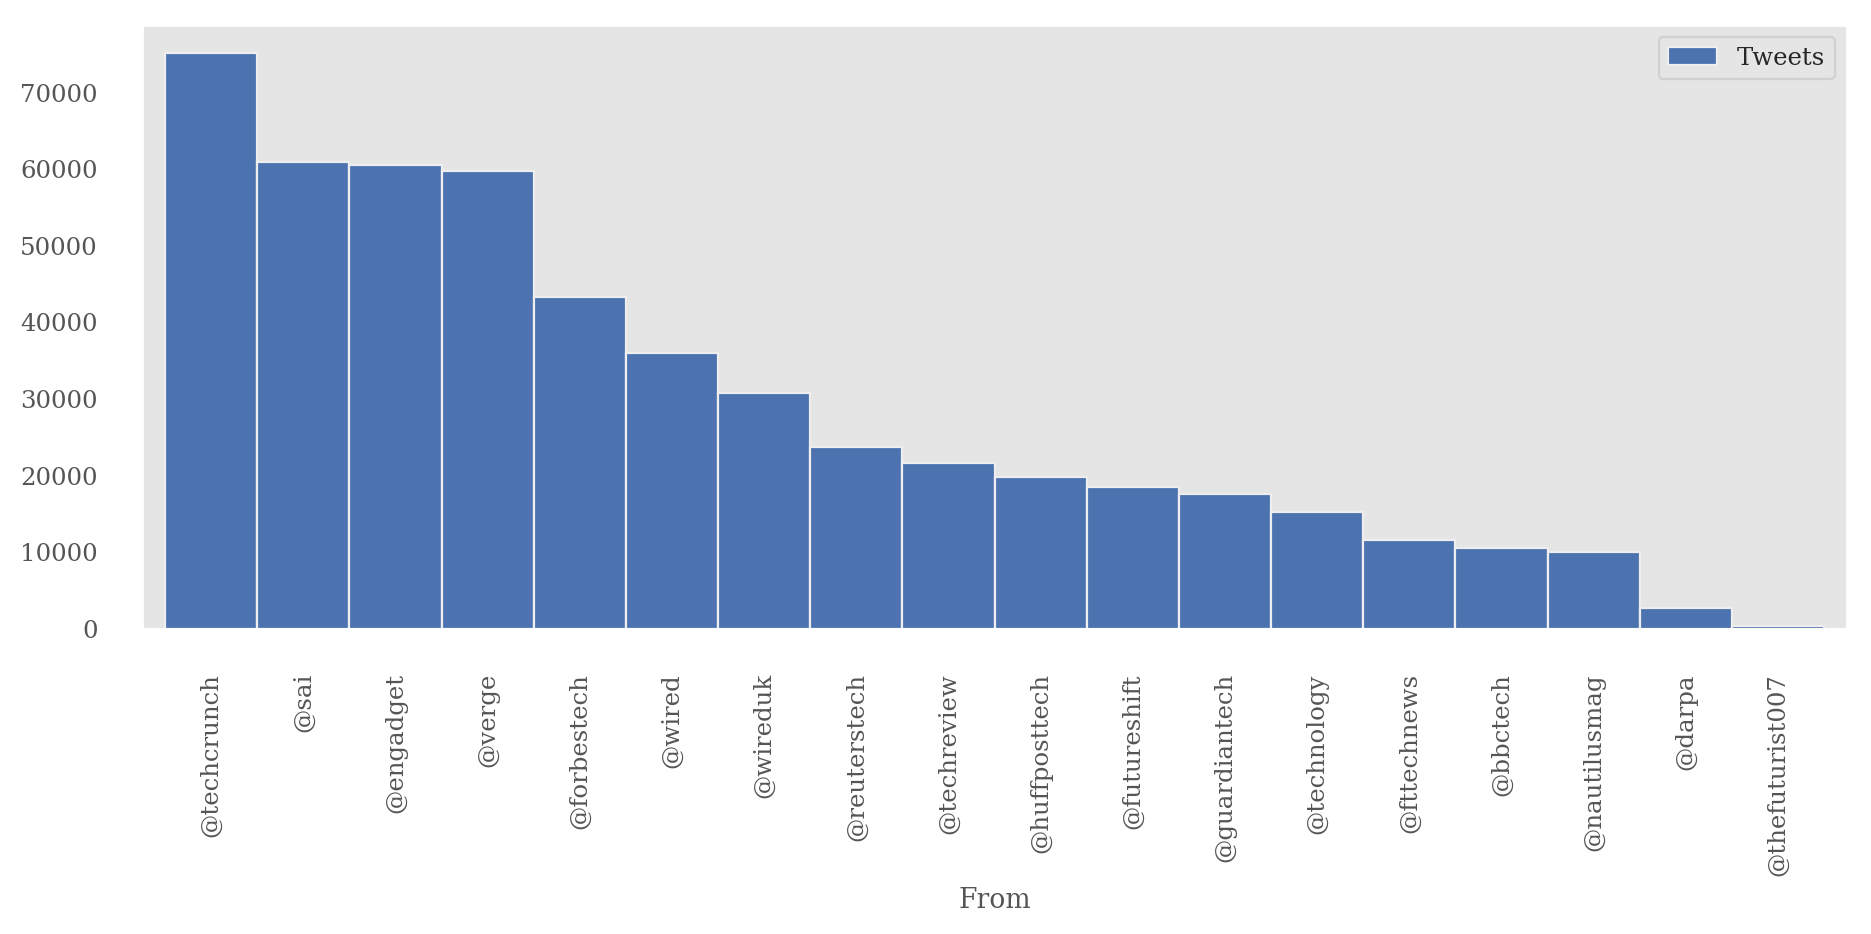
\includegraphics[width=\textwidth]{from}
		\label{fig:from}
  \end{minipage}
  \hfill
  \begin{minipage}[t]{0.4\textwidth}
		\caption{Tweets por dia.}
		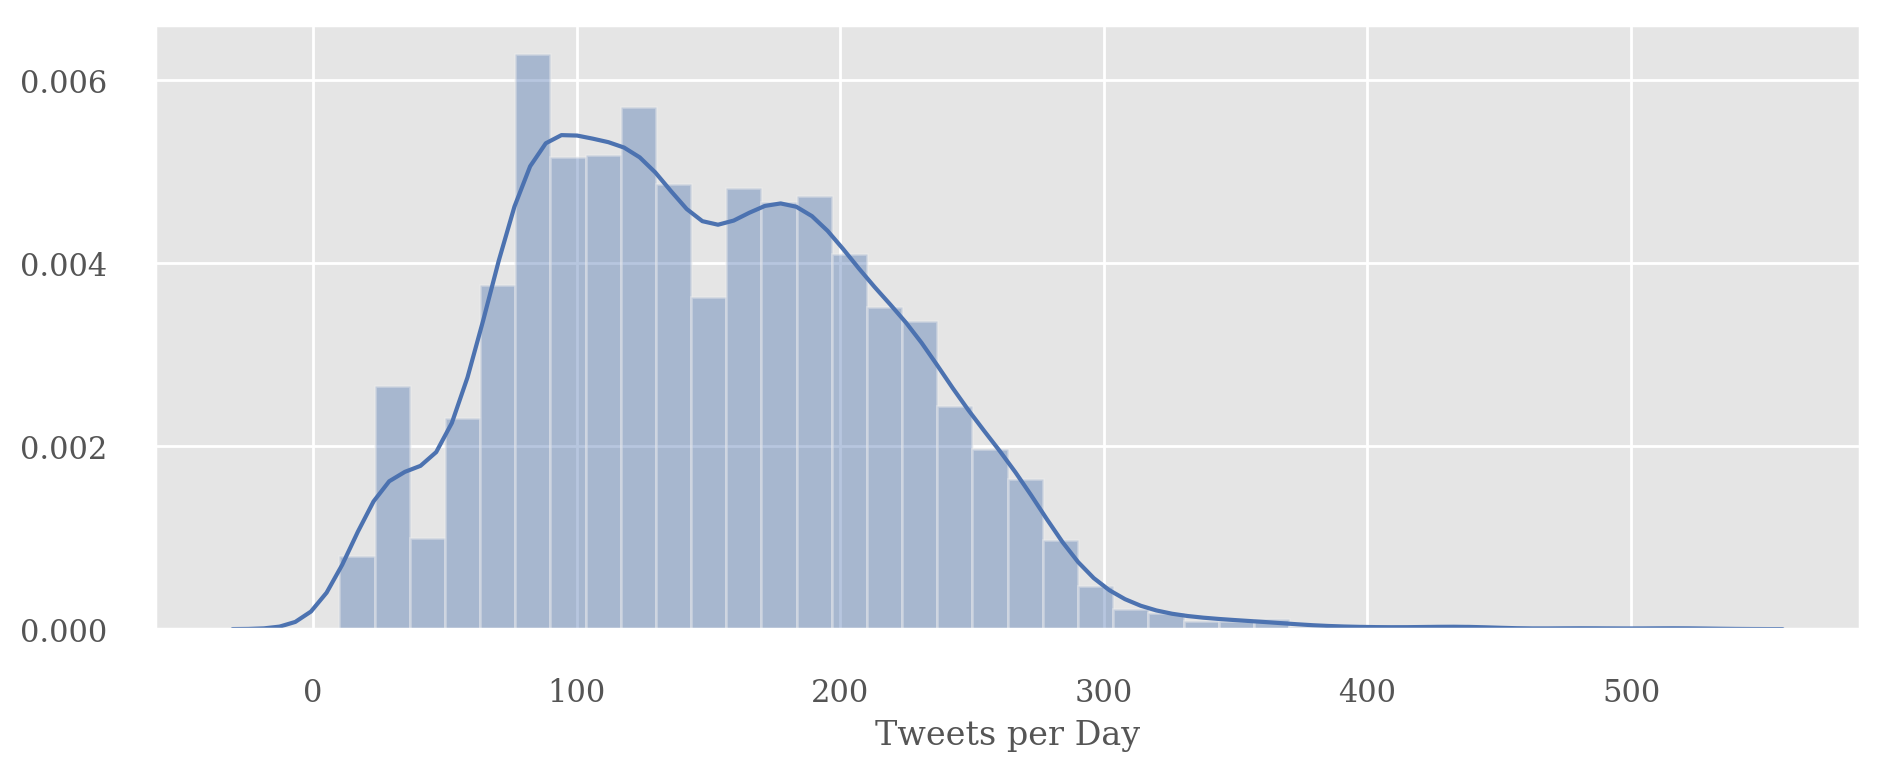
\includegraphics[width=\textwidth]{perDay}
		\label{fig:daily}
  \end{minipage}
\end{figure}
\begin{figure}[!h]
	\centering
	\caption{Tweets por período.}
	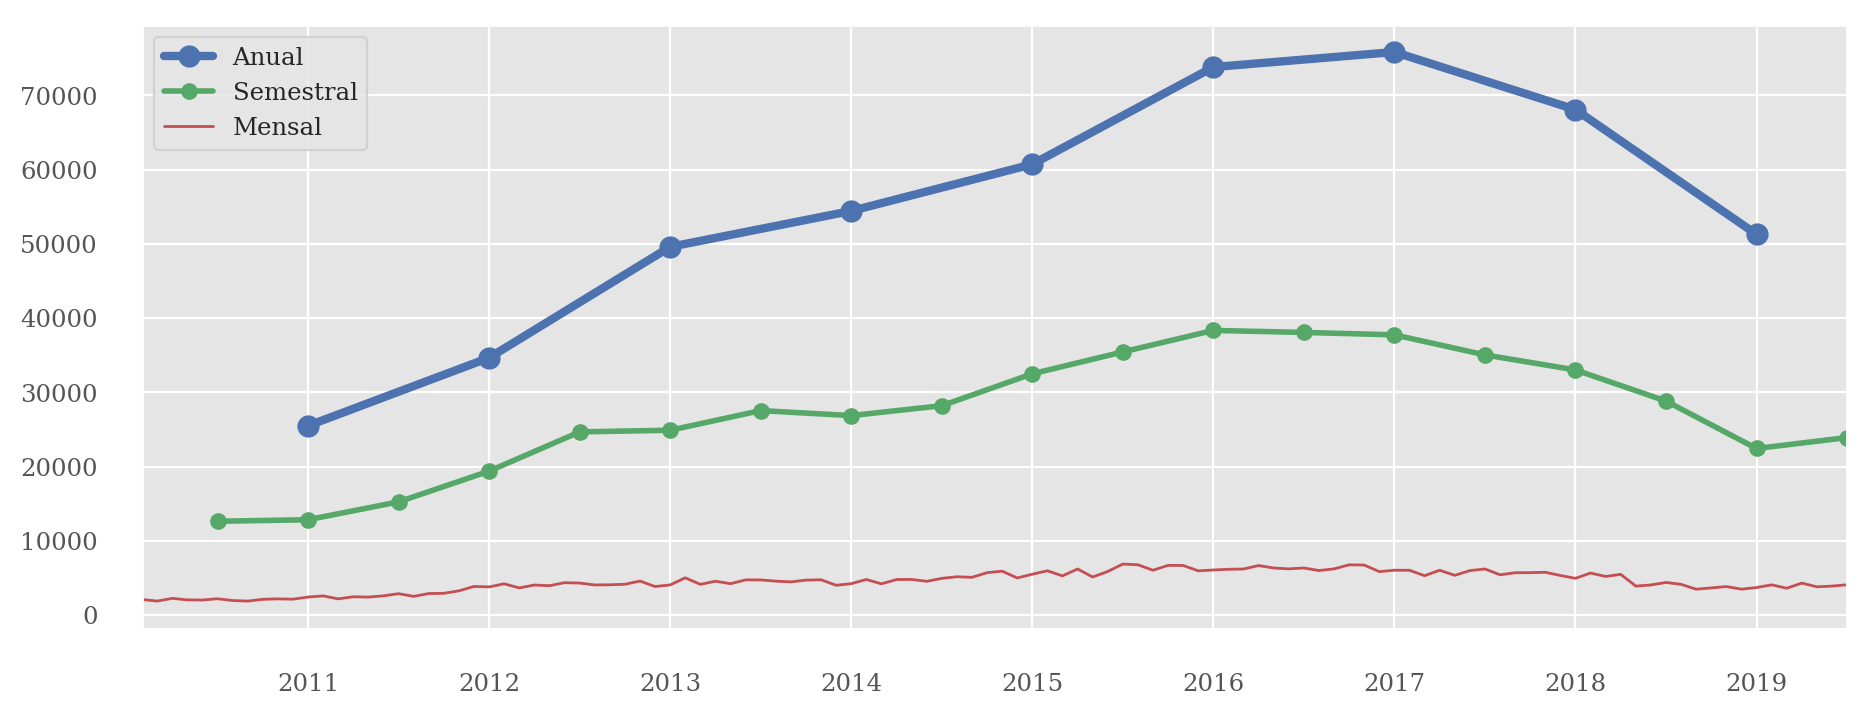
\includegraphics[width=.8\columnwidth]{anual-semestral}
	\label{fig:volume-tweets}
\end{figure}
Nosso corpus foi captado de uma seleção de contas no \emph{Twitter} notórias por cobrirem assuntos de tecnologia (ver figura \ref{fig:from}). Ao todo, foram coletadas 518.145 mensagens curtas entre janeiro de 2010 e 30 de junho de 2019, uma média entre 100 e 200 mensagens por dia (figura \ref{fig:daily}).
Há uma grande variação de tweets/smestre no período, conforme é possível notar na figura \ref{fig:volume-tweets}.
\section{Código}
\subsection{Acesso}
O código é aberto e seu repositório está disponível online no Github\footnote{http://github.com/fredguth/ipea-techmonitor}.
\subsection{Organização}
Ao clonar o reposítório, o usuário se depara com a seguinte estrutura de arquivos:
\dirtree{%
.1 ipea-techmonitor.
.2 /data.
.3 twitter.csv.
.2 /docs.
.3 data\_preparation.ipynb.
.3 generate\_trends.ipynb.
.2 config.ini.
.2 data\_preparation.py.
.2 generate\_trends.py.
.2 readme.md.
.2 requirements.txt.
.2 run.py.
}
\vspace{.7cm}
No diretório raiz encontram-se:
\begin{itemize}
	\item \textbf{config.ini}:arquivo de configuração, onde o usuário pode alterar todos os parâmetros de execução.
	\item \textbf{data\_preparation.py}: responsável pelo processo de limpeza dos dados, tokenização e geração de bigramas.
	\item \textbf{generate\_trends.py}: responsável pela criação da matriz semestre-tópico, análise estátistica e geração do arquivo de saída Excel.
	\item \textbf{readme.md}: instruções para instalação e uso do sistema.
	\item \textbf{requirements.txt}: lista de dependências python do projeto. 
	\item \textbf{run.py}: pequeno programa que apenas chama \textbf{data\_preparation.py} e \textbf{generate\_trends.py} em ordem.
\end{itemize}	
\subsection{Instalação e Uso}

\subsubsection{Instalação}
A partir do terminal de linha de comando:
\begin{lstlisting}[language=bash, frame=leftline, basicstyle=\footnotesize\ttfamily] 
git clone https://github.com/fredguth/ipea-techmonitor
pip install -r requirements.txt
\end{lstlisting}

\subsubsection{Uso}
Verifique e altere os parâmetros da execução no arquivo texto \textbf{config.ini}\label{config.ini}
\lstinputlisting[language=python, basicstyle=\footnotesize\ttfamily, lastline=24, caption={Arquivo de configuração config.ini}, frame=leftline]{../config.ini}
Quando estiver satisfeito com os parâmetros, execute na linha de comando:
\begin{lstlisting}[language=bash, frame=leftline,basicstyle=\footnotesize\ttfamily] 
python run.py
\end{lstlisting}

\bibliography{references.bib}
\bibliographystyle{chicago}
%%% End document
\end{document}